\chapter{度規、膨脹與初步宇宙學}

前一講結束時，我們已得到一個洛倫茲不變的波動方程，正準備把麥克斯威方程組寫成時空形式。現在，在轉向引力之前，一位聽眾的提問提醒我們：對稱性本身能決定物理理論的多少內容？答案很明確：能決定很多，但不是全部。洛倫茲不變性是篩選可能定律的有力條件，但不能取代其餘物理假設或實驗。

\section{對稱性無法決定的部分}

\begin{classroomqa}
\audiencequestion{既然已知電場和磁場會在洛倫茲變換下共同變換，麥克斯威方程組是否就能單憑相對論推出？}
\lecturerresponse{不能。相對論限制了方程的形式，但建構方程時還用到了線性、導數階數較低、場的變換方式，以及實驗資訊。缺少這些額外條件，仍然可能有許多洛倫茲協變的場方程。}
\end{classroomqa}

在開頭的討論中，最重要的額外假設是線性。若\(A(x,t)\)是某個線性場方程的解，則對任意常數\(\lambda\)，\(\lambda A(x,t)\)也會是解。若\(A\)和\(B\)都是解，則\begin{equation}
  C(x,t)=A(x,t)+B(x,t).
  \label{eq:superposition}
\end{equation}也是解。這就是疊加原理。兩列無源電磁波可以交會後各自保持原狀，不會像物質物體那樣直接碰撞。它們可以透過帶電物質間接相互作用，因為每列波都會推動電荷，而運動中的電荷會輻射；但真空場方程本身是線性的。

\begin{figure}[H]
\centering
\includegraphics[width=0.64\textwidth]{lecture_08_figure_01.png}
\caption{討論疊加原理時畫在黑板上的兩個波形。兩者相加後仍是允許的無源波。}
\lectureframe{00:05:30}
\end{figure}

諧振子讓這套代數關係一目了然。假設\begin{equation}
  m\ddot x=-kx.
  \label{eq:linear-oscillator}
\end{equation}。若\(x_1\)和\(x_2\)都滿足\eqref{eq:linear-oscillator}，則\begin{equation}
  m(\ddot x_1+\ddot x_2)
  =-k(x_1+x_2),
\end{equation}，所以\(x_1+x_2\)也是解。不過，若加入非線性項\begin{equation}
  m\ddot x=-kx+p x^2,
  \label{eq:nonlinear-oscillator}
\end{equation}，兩者之和就不再成立：\begin{equation}
  (x_1+x_2)^2=x_1^2+x_2^2+2x_1x_2.
\end{equation}。交叉項\(2x_1x_2\)在兩個各自的方程中都沒有對應項。此時，兩種運動便會互相影響。

\begin{figure}[H]
\centering
\includegraphics[width=0.73\textwidth]{lecture_08_figure_02.png}
\caption{比較兩個振子各自的方程與其和所滿足的方程。二次項顯示出額外的交叉項，因而破壞疊加原理。}
\lectureframe{00:10:10}
\end{figure}

這個例子確立了一項方法論要點，整段宇宙學討論都會沿用：對稱性告訴我們哪些量可以組合，以及哪些方程形式是允許的；動力學和觀測則告訴我們自然界採用的是哪一個允許的方程。

\section{間隔即幾何}

現在我們離開電磁學，簡要進入廣義相對論與宇宙學。起點是相鄰事件之間的間隔。以四維座標\(x^\mu\)標記一個事件，並以\(x^\mu+dx^\mu\)標記鄰近事件。在慣性笛卡兒座標中，採用\(c=1\)和\((+,-,-,-)\)的號差約定，\begin{equation}
  d\tau^2
  =dt^2-dx^2-dy^2-dz^2
  =dx^\mu dx_\mu
  =\eta_{\mu\nu}\,dx^\mu dx^\nu.
  \label{eq:minkowski-interval}
\end{equation}。不變的是\(d\tau^2\)，而不是任何單一座標差。洛倫茲變換會改變\(dt,dx,dy,dz\)，但會保留這個二次組合。因此，狹義相對論也可以理解為閔可夫斯基時空的幾何。

\begin{figure}[H]
\centering
\includegraphics[width=0.72\textwidth]{lecture_08_figure_03.png}
\caption{閔可夫斯基間隔依序以分量、縮併指標和度規張量的記號表示。}
\lectureframe{00:14:50}
\end{figure}

\eqref{eq:minkowski-interval}的簡單形式取決於座標選擇。即使是平坦平面，若座標標記得不恰當，係數也可能變得不熟悉。假設\(x\)以公分測量，而\(y\)以公尺測量。對於一個物理位移，\begin{equation}
  ds^2=dx^2+\left(\frac{dy}{100}\right)^2
      =dx^2+10^{-4}dy^2.
  \label{eq:mixed-units}
\end{equation}。因子\(10^{-4}\)與曲率無關，只是用來換算單位。

\begin{figure}[H]
\centering
\includegraphics[width=0.59\textwidth]{lecture_08_figure_04.png}
\caption{以公分標記一個軸、以公尺標記另一個軸的平坦平面。不相同的度規係數反映的是單位，而非曲率。}
\lectureframe{00:20:10}
\end{figure}

斜座標會引入混合項。在二維中，最一般的局部二次型可寫成\begin{align}
  ds^2
  &=a_{11}\,dx^2+a_{12}\,dx\,dy\notag\\
  &\quad+a_{21}\,dy\,dx+a_{22}\,dy^2,
  \qquad a_{12}=a_{21}.
  \label{eq:quadratic-form}
\end{align}。由於普通微分可以交換，\(dx\,dy=dy\,dx\)，只有係數陣列的對稱部分會有貢獻。我們把係數整理成矩陣\begin{equation}
  g=
  \begin{pmatrix}
    a_{11} & a_{12}\\
    a_{21} & a_{22}
  \end{pmatrix}.
  \label{eq:metric-matrix}
\end{equation}。這個矩陣就是\emph{度規}，它是將座標差轉換為物理間隔的局部規則。

\begin{figure}[H]
\centering
\includegraphics[width=0.71\textwidth]{lecture_08_figure_05.png}
\caption{二次微分形式，以及其對稱的\(2\times2\)係數矩陣；此處正是將該矩陣辨認為度規之時。}
\lectureframe{00:24:07}
\end{figure}

均勻的矩形或斜交網格會給出常數係數。如果座標線彎曲、逐漸密集或逐漸疏開，即使底層曲面仍然平坦，這些係數也會成為位置的函數。一般的時空記號是
\begin{equation}
  ds^2=g_{\mu\nu}(x)\,dx^\mu dx^\nu.
  \label{eq:general-metric}
\end{equation}

\begin{figure}[H]
\centering
\includegraphics[width=0.66\textwidth]{lecture_08_figure_06.png}
\caption{座標網格可以隨位置改變後的一般位置相依度規。}
\lectureframe{00:28:10}
\end{figure}

在指定的座標系中知道\(g_{\mu\nu}\)，便能確定局部距離、時間和角度，進而確定幾何。反過來則不唯一：同一幾何有無窮多種座標描述，因此也有無窮多組由座標變換彼此關聯的係數函數。

\section{座標複雜性與內在曲率}

現在必須區分複雜的度規與彎曲的空間。把一張紙捲成圓柱，不要拉伸它。紙在房間中的外觀變了，但在紙面上測得的所有距離都保持不變。被限制在紙面上的生物，無法透過任何內在測量察覺這種彎曲。這是外在彎曲，並非這裡所說的曲率。

半球則不同。不拉伸、不撕裂或不壓縮，就無法把它壓平。地球的平面地圖必然會扭曲距離、面積、角度，或它們的某種組合。這種限制是內在的，不必觀察周圍維度就能測出。

極座標提供了一個不可或缺的平坦反例。在平面上，無窮小的徑向位移長度為\(dr\)；在半徑\(r\)處，角位移\(d\theta\)的長度則為\(r\,d\theta\)。因此
\begin{equation}
  ds^2=dr^2+r^2d\theta^2,
  \qquad
  g_{\text{polar}}=
  \begin{pmatrix}
    1&0\\
    0&r^2
  \end{pmatrix}.
  \label{eq:polar-metric}
\end{equation}
係數\(r^2\)雖然在平面上隨位置改變，平面本身仍是平坦的。經由變數變換
\begin{equation}
  x=r\cos\theta,\qquad y=r\sin\theta
\end{equation}
便可回到常數度規\(ds^2=dx^2+dy^2\)。

\begin{figure}[H]
\centering
\includegraphics[width=0.70\textwidth]{lecture_08_figure_07.png}
\caption{極座標度規及其轉回笛卡兒度規的形式。左側的位置相依矩陣描述的仍是平坦平面。}
\lectureframe{00:39:20}
\end{figure}

\begin{classroomqa}
\audiencequestion{極座標中的角向距離是否應該包含正弦？}
\lecturerresponse{平面上不需要。那裡的弧長是\(r\,d\theta\)。正弦項出現在球面上，因為緯圈的半徑是\(R\sin\theta\)。}
\end{classroomqa}

取半徑為\(R\)的球面。令\(\theta\)為自北極量起的極角，\(\phi\)為方位角。沿子午線移動一小段的長度為\(R\,d\theta\)。在極角\(\theta\)處，緯圈半徑為\(R\sin\theta\)，因此沿方位角移動一小段的長度為
\(R\sin\theta\,d\phi\)。由局部的畢氏定理可得
\begin{align}
  ds^2
  &=R^2\left(d\theta^2+\sin^2\theta\,d\phi^2\right),
  \label{eq:sphere-metric}\\
  g_{\text{sphere}}=
  &\begin{pmatrix}
    R^2&0\\
    0&R^2\sin^2\theta
  \end{pmatrix}.
\end{align}

\begin{figure}[H]
\centering
\includegraphics[width=0.72\textwidth]{lecture_08_figure_08.png}
\caption{球面、其角向線元素，以及相應的度規矩陣。因子\(\sin^2\theta\)反映緯圈半徑逐漸縮小。}
\lectureframe{00:45:15}
\end{figure}

\begin{figure}[H]
\centering
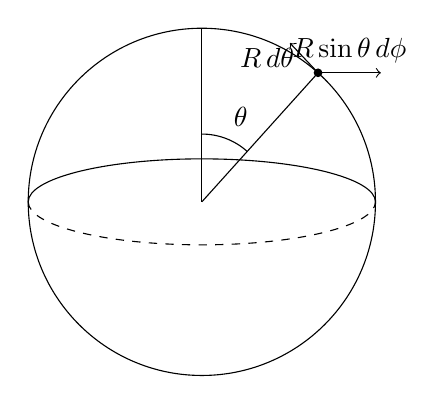
\begin{tikzpicture}[scale=1.05]
  \draw (0,0) circle (2.1);
  \draw[dashed] (-2.1,0) arc (180:360:2.1 and 0.52);
  \draw (2.1,0) arc (0:180:2.1 and 0.52);
  \coordinate (P) at (48:2.1);
  \fill (P) circle (1.5pt);
  \draw (0,0) -- (0,2.1);
  \draw (0,0) -- (P);
  \draw (0,0.82) arc (90:48:0.82);
  \node at (0.47,1.03) {\(\theta\)};
  \draw[->] (P) -- ++(-0.34,0.36)
    node[midway,left] {\(R\,d\theta\)};
  \draw[->] (P) -- ++(0.76,0)
    node[midway,above] {\(R\sin\theta\,d\phi\)};
\end{tikzpicture}
\caption{用來推導\eqref{eq:sphere-metric}的局部微分線段示意圖，經重新清楚繪製。}
\end{figure}

不存在任何全域座標變換，能將\eqref{eq:sphere-metric}化為常數的歐幾里得矩陣。二維觀測者可以透過內在測量發現這點：由測地線構成的足夠大三角形，內角和會大於\(180^\circ\)。至此可得到一項實用判準：係數變化本身並不代表有曲率。曲率意味著，在所考慮的區域內，無法找到一組座標使度規處處為常數。

\section{從彎曲時空到宇宙學}

廣義相對論允許時空本身具有這種內在曲率。位置相依的\(g_{\mu\nu}\)仍可能只是座標造成的表象，如同極座標的情況；但在真正彎曲的時空中，沒有任何座標變換能在全域上消除這種變化。

\begin{figure}[H]
\centering
\includegraphics[width=0.70\textwidth]{lecture_08_figure_09.png}
\caption{從特殊座標的例子轉向一般時空線元素\(ds^2=g_{\mu\nu}(x)dx^\mu dx^\nu\)。}
\lectureframe{00:48:40}
\end{figure}

我們不打算探討愛因斯坦方程的完整架構，而是把討論限於適用於宇宙學的幾何：空間在足夠大的尺度上視為均勻，但幾何可以隨時間改變。均勻表示沒有任何位置異於其他位置。這不代表平坦：球面上每一點都等價，但球面仍是彎曲的；也不代表每個尺度上都毫無結構。

\begin{classroomqa}
\audiencequestion{既然星系會形成星系團、片狀結構和絲狀結構，宇宙怎麼會是均勻的？}
\lecturerresponse{這個說法適用於粗粒化後的尺度。恆星、星系和星系團都高度不均勻。比較橫跨數億光年的區域時，這些結構平均後會趨近均勻分布。宇宙學原理是依據經驗採用的工作假設，並非邏輯上的必然；如果發現足夠大的系統性差異，包括宇宙背景輻射的方向差異，就可能推翻這項假設。}
\end{classroomqa}

本講的第二項大尺度假設是空間平坦。在固定的宇宙時刻，足夠大的三角形看來符合歐幾里得幾何：內角和為\(180^\circ\)。這是對三維空間幾何的描述，尚未涉及四維時空的曲率。

\begin{classroomqa}
\audiencequestion{相隔宇宙學距離的點之間，如何定義同時性？它們發出的光是在不同時刻抵達我們這裡的。}
\lecturerresponse{我們無法在遙遠星系之間放置量尺，也無法在同一瞬間觀察它們。我們在較晚的時刻收到訊號，再依據時空模型重建發射事件的幾何。這個過程是間接的，但天文學中許多幾何測量也都是如此。所謂平坦，是指在調查的尺度上，重建出的巨大三角形沒有可測得的角盈餘或角虧損。}
\end{classroomqa}

\section{共動座標與尺度因子}

想像在星系的大尺度流動上畫一張笛卡兒網格。網格膨脹時，每個星系都維持原有的座標標記。這個標記不是以公尺為單位的距離，而是一個位置地址。隨時間改變的換算因子，會把座標間隔轉換為物理間隔。

\begin{figure}[H]
\centering
\begin{tikzpicture}[>=Latex,scale=0.86]
  \foreach \x in {0,0.65,1.3,1.95,2.6} {
    \draw[gray!65] (\x,0) -- (\x,2.2);
  }
  \foreach \y in {0,0.55,1.1,1.65,2.2} {
    \draw[gray!65] (0,\y) -- (2.6,\y);
  }
  \fill[blue!65!black] (0.65,0.55) circle (2pt);
  \fill[red!70!black] (1.95,1.65) circle (2pt);
  \node[below] at (1.3,-0.2) {comoving labels at \(t_1\)};
  \draw[->,very thick] (3.0,1.1) -- (4.0,1.1)
    node[midway,above] {\(a(t)\) grows};
  \foreach \x in {4.4,5.5,6.6,7.7,8.8} {
    \draw[gray!65] (\x,0) -- (\x,2.2);
  }
  \foreach \y in {0,0.55,1.1,1.65,2.2} {
    \draw[gray!65] (4.4,\y) -- (8.8,\y);
  }
  \fill[blue!65!black] (5.5,0.55) circle (2pt);
  \fill[red!70!black] (7.7,1.65) circle (2pt);
  \node[below] at (6.6,-0.2) {same labels at \(t_2\)};
\end{tikzpicture}
\caption{共動位置標記保持固定，座標網格的物理間距則逐漸增大。}
\end{figure}

空間均勻性要求在同一時刻，各處的換算因子都相同。空間平坦性則允許度規的空間部分採用笛卡兒形式。於是線元素為
\begin{equation}
  d\tau^2
  =dt^2-a^2(t)\left(dx^2+dy^2+dz^2\right).
  \label{eq:flrw-flat}
\end{equation}
這就是共動座標下，空間平坦且均勻的宇宙學度規。我們可以令\(x,y,z\)無量綱，並讓\(a(t)\)具有長度單位。也可以採用另一種約定，把量綱放在座標中，使\(a\)無量綱；只有兩者的乘積有意義。

\begin{figure}[H]
\centering
\includegraphics[width=0.76\textwidth]{lecture_08_figure_10.png}
\caption{黑板上完成的空間平坦宇宙學度規，共同因子\(a^2(t)\)乘在三個空間方向上。}
\lectureframe{01:03:15}
\end{figure}

如果\(a\)是常數，就可以藉由重新縮放\(x,y,z\)將它吸收，而\eqref{eq:flrw-flat}便是單位不同的普通閔可夫斯基時空。真正非平凡之處在於它隨時間變化。

\begin{classroomqa}
\audiencequestion{如果座標網格在膨脹，為什麼米尺、原子和星系不跟著膨脹？}
\lecturerresponse{度規描述的是宇宙的平均流動，並非迫使每個束縛系統隨之運動的力。電磁力使米尺和原子維持在一起；自引力則束縛星系。在小尺度上，這些束縛效應遠勝於極微弱的背景膨脹。鄰近星系也可能偏離哈伯流：仙女座星系正受到銀河系吸引。對星系束縛的詳細研究顯示，僅靠可見物質並不足夠；這是支持暗物質存在的論據之一。}
\end{classroomqa}

\begin{classroomqa}
\audiencequestion{為什麼尺度因子本身不是把星系推開的力？}
\lecturerresponse{依照目前的約定，它的量綱是長度，不是力。想想一顆向上發射的砲彈：發射之後，它向外運動是慣性的；引力則藉由降低其速度或將它拉回來改變這種運動。同樣地，膨脹是一種運動狀態。動力學所要回答的是引力與其他來源如何改變\(\dot a\)和\(\ddot a\)，而不是需要什麼力才能讓\(a\)持續運動。}
\end{classroomqa}

過去人們預期，吸引性的引力應使膨脹減速。到本講進行時，天文證據已顯示近期的宇宙膨脹反而正在加速，這表示完整的動力學不只包含一般的吸引性物質。等幾何架構確立後，我們再討論這個問題。

\section{哈伯定律}

取兩個共動星系，它們的座標間隔固定為
\(\Delta x\)。在同一宇宙時刻，它們的物理距離為
\begin{equation}
  D(t)=a(t)\,\Delta x.
  \label{eq:physical-distance}
\end{equation}
保持共動位置標記不變，對時間微分：
\begin{align}
  V(t)
    &=\dot D(t)
      =\dot a(t)\,\Delta x \nonumber\\
    &=\frac{\dot a(t)}{a(t)}D(t).
  \label{eq:hubble-derivation}
\end{align}
定義
\begin{equation}
  H(t)=\frac{\dot a(t)}{a(t)}.
  \label{eq:hubble-parameter}
\end{equation}
於是
\begin{equation}
  V(t)=H(t)D(t).
  \label{eq:hubble-law}
\end{equation}
在同一宇宙時刻，\(H(t)\)必須處處相同，否則空間就不均勻。退行速度與距離成正比，因為共動網格中的每段間隔都以相同的相對速率伸展。

\begin{figure}[H]
\centering
\includegraphics[width=0.73\textwidth]{lecture_08_figure_11.png}
\caption{物理距離\(D=a\Delta x\)及其時間導數，逐步推導出\(V=(\dot a/a)D\)。}
\lectureframe{01:16:45}
\end{figure}

\begin{classroomqa}
\audiencequestion{對遙遠星系而言，哈伯參數應取現在的值，還是觀測到的光發出時的值？}
\lecturerresponse{應取所描述時期的值。來自遙遠星系的光讓我們得知較早時期的膨脹狀況。嚴謹的分析必須考慮\(H\)隨時間的變化；處處代入今天的值，只是局部近似。}
\end{classroomqa}

\begin{classroomqa}
\audiencequestion{在\(D=a\Delta x\)中，單位包含在哪裡？}
\lecturerresponse{一種方便的選擇，是把共動位置標記\(\Delta x\)視為無量綱，並讓\(a\)帶有長度單位。也可以採用相反的記帳方式。無論怎麼選，\(H=\dot a/a\)的量綱都是時間的倒數。}
\end{classroomqa}

\section{膨脹座標中的光}

光沿著零路徑傳播。沿此路徑，固有時間間隔為零：
\begin{equation}
  d\tau^2=0.
\end{equation}

\begin{classroomqa}
\audiencequestion{為什麼光的間隔為零？}
\lecturerresponse{這是相對論中光線的定義性幾何。每個局部自由落下的觀測者都測得光以\(c=1\)運動，因此局部有\(dt^2=d\ell^2\)，時空間隔也就為零。這不表示接收光的觀測者沒有經歷座標時間。}
\end{classroomqa}

對只沿\(x\)方向移動的光線，
\begin{equation}
  0=dt^2-a^2(t)\,dx^2.
\end{equation}
選擇沿\(x\)增加方向移動的光線，
\begin{equation}
  dt=a(t)\,dx,
  \qquad
  dx=\frac{dt}{a(t)},
  \qquad
  \frac{dx}{dt}=\frac{1}{a(t)}.
  \label{eq:null-ray}
\end{equation}

\begin{figure}[H]
\centering
\includegraphics[width=0.64\textwidth]{lecture_08_figure_12.png}
\caption{膨脹度規中的零條件，以及由此得到的共動光線方程\(dx=dt/a(t)\)。}
\lectureframe{01:23:45}
\end{figure}

尺度因子增大時，座標速度\(dx/dt\)會減小。這不表示光在局部變慢。一單位的共動座標距離所代表的物理距離愈來愈大，因此座標速度的數值會改變，但局部測量仍都得到\(c=1\)。

\section{時間依賴性為何重要}

現在無可迴避的核心幾何問題是：\(a(t)\)如何變化？這就像已知某個拋射體在一個時刻的位置；要知道它未來的軌跡，還需要運動方程。在宇宙學中，引力動力學會提供描述\(a(t)\)的方程。

\begin{classroomqa}
\audiencequestion{為什麼要特別關注\(a(t)\)是否隨時間變化，卻不提出同樣合理的問題，例如電子電荷是否隨時間變化？}
\lecturerresponse{兩者沒有邏輯上的優先次序。若測得電子電荷變化，那將極為重要。我們聚焦於\(a(t)\)，是因為觀測已告訴我們宇宙間距正在改變，而電子電荷看來保持不變。從幾何角度看，恆定的\(a\)可以藉由改變空間單位而消去，留下平坦時空；隨時間變化的\(a\)則無法用這種方式消去。}
\end{classroomqa}

要測量遙遠星系的退行，必須先有這套幾何架構，才能說清楚我們究竟在測量什麼。最粗略地說，已知光度的光源會因距離而顯得較暗，因為光分散到更大的面積上；已知原子譜線的位置偏移則給出紅移，作為退行的指標。哈伯將距離估計與紅移結合，發現了正比關係\eqref{eq:hubble-law}，不過早期所得的係數數值差距相當大。現代的距離階梯和相對論光傳播計算精細得多，但概念上仍是以距離和紅移相互配合。

\section{哈伯時間與宇宙年齡估計}

哈伯定律隱含著一個簡單的估算方法：把星系目前的退行速度固定不變，假設它以均勻速度倒退。它回到目前距離所需的時間為
\begin{equation}
  t=\frac{D}{V}.
\end{equation}
利用\(V=HD\)，
\begin{equation}
  t=\frac{D}{HD}=\frac{1}{H}.
  \label{eq:hubble-time}
\end{equation}
距離會相消，因此任意一對共動星系都給出相同的粗略時間。Susskind在這裡指出並更正了一個容易說錯的地方。假設並不是\(H\)保持不變，而是把該星系的退行速度視為固定值，並向過去外推。

\begin{figure}[H]
\centering
\includegraphics[width=0.66\textwidth]{lecture_08_figure_13.png}
\caption{哈伯時間估算\(H^{-1}=D/(HD)=D/V\)：向過去外推時，距離會相消。}
\lectureframe{01:33:45}
\end{figure}

哈伯參數的倒數因此是一個時間尺度，但不一定就是宇宙的精確年齡。在純粹減速、由物質主導的圖像中，將目前速度反向，再讓引力把星系拉回。它們會比以均勻速度運動時更早相遇，因此目前的\(H^{-1}\)會高估宇宙年齡。本講引用較精確的估計，約為\(13.5\)億年，與哈伯時間接近但並不相同。

\begin{classroomqa}
\audiencequestion{如果我們的星系內部沒有哈伯膨脹，把所有星系反向推演到坍縮又是什麼意思？}
\lecturerresponse{均勻模型終究無法再描述束縛結構的真實歷史。沿時間正向演化時，小幅漲落會在引力作用下成長為星系和星系團。若真的把電影倒轉，就必須反轉每一個微觀運動，並使熵減少；單是反轉平均哈伯流，並不能讓已形成的結構消失。向過去外推是粗略的宇宙學估算，並非讓每顆恆星沿原路倒退的影片。}
\end{classroomqa}

\begin{classroomqa}
\audiencequestion{實驗能否分辨星系際距離正在增加，還是尺子正在縮短？}
\lecturerresponse{只有無量綱比值可以觀測。測得的是星系間距除以原子或實驗室長度標準後的比值增加。我們通常假設原子和分子物理的參數固定，並說宇宙正在膨脹。也可以選星系際間距作為標準，描述原子、質子和米尺正在縮短。這個比值所代表的物理不會改變。}
\end{classroomqa}

這種約定很自然，因為尺子由原子構成，其大小由看似恆定的參數決定。歸根究柢，一公尺是許多微觀長度的總和。固定這些微觀標準，就得到熟悉的說法：\(a(t)\)在增長。

\begin{classroomqa}
\audiencequestion{\eqref{eq:flrw-flat}是唯一與空間均勻和平坦相容的度規嗎？}
\lecturerresponse{若只差在座標變換，則可以這麼說。更精確地說，在這些假設下，適當選擇宇宙時間與共動空間座標後，度規可以化為這種形式。另一種座標系可能會讓同一時空看起來很不一樣。}
\end{classroomqa}

\begin{classroomqa}
\audiencequestion{當向過去推演的星系間距降至零時，哈伯定律也給出零速度。這是否會使星系無法相遇？}
\lecturerresponse{不會。今天推得的\(H\)並非一路向過去都保持不變。在一般的膨脹解中，\(H(t)\)在較早時期大得多。估算\(H_0^{-1}\)時，只是把今天的速度均勻外推，用來取得一個時間尺度；真正的\(a(t)\)、\(H(t)\)和速度都必須由動力學求得。}
\end{classroomqa}

\section{牛頓殼層定理與宇宙學動力學}

要找出動力學，先把星系平滑成均勻介質。選一個星系作為原點，另一個星系的共動座標標記為\(x\)。這個選擇沒有特殊的物理地位；均勻性要求最後得到的方程以任何星系為中心都相同。第二個星系的物理半徑為
\begin{equation}
  R(t)=a(t)x.
  \label{eq:radius-ax}
\end{equation}

起初，要計算它的引力加速度，似乎得加總巨大宇宙中每個星系的吸引力。牛頓殼層定理將問題簡化如下：

\begin{proposition}[Newton's shell theorem]
對於反平方定律的力和球對稱的質量分布，通過測試點的球面之外的物質，合力為零。球面之內的物質對測試點的作用，等同於所有包圍在內的質量都集中在球心。
\end{proposition}

\begin{figure}[H]
\centering
\includegraphics[width=0.70\textwidth]{lecture_08_figure_14.png}
\caption{均勻分布的星系、位於共動座標\(x\)處的測試星系，以及一個球面；只有球面內的質量會影響測試星系的徑向運動。}
\lectureframe{01:50:05}
\end{figure}

\begin{figure}[H]
\centering
\begin{tikzpicture}[scale=0.94,>=Latex]
  \draw[gray!65] (0,0) circle (2.35);
  \foreach \p in {
    (-1.5,0.8),(-1.2,-0.8),(-0.8,1.5),(-0.6,0.35),(-0.3,-1.45),
    (0.15,1.05),(0.35,-0.55),(0.7,1.65),(0.9,0.45),(1.25,-0.9),
    (1.65,0.95),(-1.75,-0.2),(1.8,-0.15)} {
    \fill[black!55] \p circle (1.15pt);
  }
  \fill[blue!65!black] (0,0) circle (2pt)
    node[below left] {chosen origin};
  \fill[red!70!black] (2.35,0) circle (2.2pt)
    node[right] {test galaxy};
  \draw[->,thick] (0,0) -- (2.32,0)
    node[midway,above] {\(R=a(t)x\)};
  \draw[<->] (-2.35,-2.55) -- (2.35,-2.55)
    node[midway,below=4pt] {only the enclosed mass contributes};
\end{tikzpicture}
\caption{殼層定理情境的清楚示意圖。原點只是方便的選擇，並非宇宙中心。}
\end{figure}

如此一來，宇宙學的多體問題便化為熟悉的單體問題：一個物體在目前球面內所包圍質量的引力下沿徑向運動。牛頓方程會決定\(R=a x\)，以及由此決定\(a(t)\)的加速度。本講刻意在進行這項計算之前停下。下一講將推導最簡單的物質主導宇宙學，不會把答案預先塞進幾何架構。

\section{最後的提問：光、大爆炸與曲率}

正式講課已經結束，但最後幾個問題揭示了幾種容易誤導人的圖像；它們屬於物理內容的一部分，並非附錄。

\begin{classroomqa}
\audiencequestion{如果來自極遙遠天體的光是在宇宙小得多時發出的，為什麼現在看起來卻是從那麼遙遠的地方傳來？如果早期宇宙很緊密，為什麼我們仍無法觀測到它的全部？}
\lecturerresponse{必須在膨脹座標中求解零光線方程。當\(a(t)\)非常小時，\(dx/dt=1/a(t)\)非常大：光在局部仍以\(c=1\)運動，卻能跨越很大的共動座標間隔。隨著\(a(t)\)增大，光的共動座標速度便會降低。精確的發射位置和可觀測區域的大小，取決於\(a(t)\)的完整演化歷史，因此要等到求解特定的宇宙學模型後，才能給出數值答案。}
\end{classroomqa}

\begin{figure}[H]
\centering
\includegraphics[width=0.72\textwidth]{lecture_08_figure_15.png}
\caption{\((x,t)\)平面中的光線：當\(a(t)\)很小時，光線在共動座標中幾乎呈水平；隨著尺度因子增大，光線逐漸變陡。}
\lectureframe{01:56:20}
\end{figure}

對\eqref{eq:null-ray}積分，就能明確寫出先前擱置的計算：
\begin{equation}
  \Delta x
  =\int_{t_{\mathrm e}}^{t_0}\frac{dt}{a(t)}.
  \label{eq:comoving-light-distance}
\end{equation}
當\(t_{\mathrm e}\)趨近宇宙開端時，這個積分是否會延伸至任意大的共動距離，取決於\(a(t)\)在早期的形式。\editorialnote{方程\eqref{eq:comoving-light-distance}是黑板上方程\(dx=dt/a(t)\)的積分形式。它明確呈現了講座留待下次課程進行的計算，且未預先選定特定的尺度因子。}

\begin{figure}[H]
\centering
\begin{tikzpicture}[scale=0.92,>=Latex]
  \draw[->] (0,0) -- (6.4,0) node[right] {\(x\)};
  \draw[->] (0,0) -- (0,4.6) node[above] {\(t\)};
  \draw[thick,blue!65!black]
    plot[smooth] coordinates {(0,0.18) (1.65,0.42) (2.65,1.05)
      (3.35,2.05) (3.85,3.25) (4.05,4.25)};
  \fill[red!70!black] (4.05,4.25) circle (2pt)
    node[right] {reception today};
  \draw[dashed] (4.05,0) -- (4.05,4.25);
  \node[align=left] at (1.65,3.25)
    {\(\displaystyle \frac{dx}{dt}=\frac1{a(t)}\)\\
     large when \(a\) is small};
\end{tikzpicture}
\caption{以共動座標清楚呈現的光線構造。斜率的變化是座標效應，並非局部光速有所改變。}
\end{figure}

\begin{classroomqa}
\audiencequestion{大爆炸是否從一個點拋出物質，因此物質現在應位於一個正在膨脹的殼層或環上？}
\lecturerresponse{不是。這個模型以均勻且密度極高的空間為起點。所有大尺度距離都在增大；物質並非從某個特定中心發射出去，穿越原本就存在的空曠空間。表面均勻布滿圓點的氣球，是一個有用的二維類比：氣球膨脹時，圓點之間的距離都會增大，而表面上的圓點分布仍然均勻。空間甚至可能在所有正時間都具有無限範圍；膨脹並不表示宇宙起初是另一個物體內部的有限球體。}
\end{classroomqa}

\begin{classroomqa}
\audiencequestion{膨脹期間，引力本身是變弱了還是變強了？}
\lecturerresponse{這裡假設牛頓常數\(G\)保持不變。儘管如此，引力仍會改變，因為距離和所含物質的密度都會改變。較早時，同一個共動星系在物理距離上更近，均勻分布的物質也更密集，因此引力造成的減速度更大。殼層定理的計算正是要量化這一點。}
\end{classroomqa}

最後，不能把空間曲率和膨脹混為一談。地球上一小塊區域看起來是平的，因為它的尺度相較於地球半徑極小。測量足夠大的三角形，就能探測角度總和的超額，或為曲率半徑設定下限。天文學以巨大的三角形進行類似的實驗。依照2006年講座採用的觀測說法，在可見區域內並未探測到曲率，因此曲率半徑必定遠大於該區域。這並不能證明宇宙完全平坦；它只能限制我們所能觀測部分的彎曲程度。

對球面而言，內在曲率按\(R^{-2}\)變化。因此，球面愈大，在局部看起來就愈平。同樣地，如果均勻宇宙具有非零的空間曲率，膨脹就會增大其曲率半徑，並降低任何固定大小的局部區域中可觀測到的曲率。
\editorialnote{\(R^{-2}\)的標度關係，以標準的定量形式表達了講座所述「球面愈大，曲率數值愈小」這一點。}

\begin{classroomqa}
\audiencequestion{如果空間是彎曲的，宇宙是否必須有一部分在收縮，而另一部分在膨脹？}
\lecturerresponse{不是。正、零或負的空間曲率，描述的是每個宇宙時間切片的幾何。膨脹或收縮則由\(a(t)\)的演化決定。彎曲的宇宙可以膨脹，平坦的宇宙也可以收縮。膨脹之後可能逆轉，就像向上運動的拋射體可能落回地面；但曲率本身並不包含同時發生的收縮。動力學上的問題是，向外的運動究竟能否逃脫所包圍質量的引力，還是會落回，抑或恰好處於臨界狀態。}
\end{classroomqa}

以逃逸速度作比較，是本講最後一個黑板上的要點。幾何已經給出了度規、哈伯定律和光線方程；牛頓定理則將動力學問題化簡為球體內的質量。下一講正好從本講應該結束之處開始：探討決定\(a(t)\)的方程，以及膨脹究竟會逃脫、再度塌縮，還是恰好處於臨界狀態。